\chapter{Un bosque hecho por factores}
\label{cap:bosque}

\begin{enpocas}
Cómo se genera cada bosque a partir de cuatro factores (oclusión, iluminación, viento y semilla), cómo
se mide la cobertura de copas y dónde se colocan las personas.
\end{enpocas}

\section{Por qué un bosque ``por factores''}

Para saber si una estrategia de búsqueda es mejor que otra hay que compararlas en condiciones
controladas: el mismo bosque, las mismas personas, cambiando una cosa a la vez. Por eso cada bosque se
genera a partir de \textbf{factores}:
\begin{description}
  \item[Oclusión] (baja, media, alta): fracción del suelo cubierta por copas, 15, 45 y 75~\%.
  \item[Iluminación] (alta, baja): sol de mediodía o sombras largas de tarde.
  \item[Viento] (no, sí): 4~m/s medios con ráfagas (\cod{WindEffects}).
  \item[Semilla:] un número que fija dónde quedan los árboles y las personas; con la misma semilla
        sale exactamente el mismo bosque.
\end{description}

\begin{lstlisting}[style=bash]
python3 scripts/generar_mundo.py --oclusion media --iluminacion alta --viento no --semilla 1 --salida ~/mundos
\end{lstlisting}

\section{Cobertura de copas}

Los robles miden 10~m de diámetro de copa y los pinos 3.2~m. El generador coloca árboles al azar y, sobre
una rejilla de 0.5~m, mide qué fracción del cuadrado de $120\times120$~m queda bajo alguna copa; se
detiene al llegar a la cobertura pedida. Deja libres 8~m alrededor del despegue.

\begin{figure}[H]
\centering
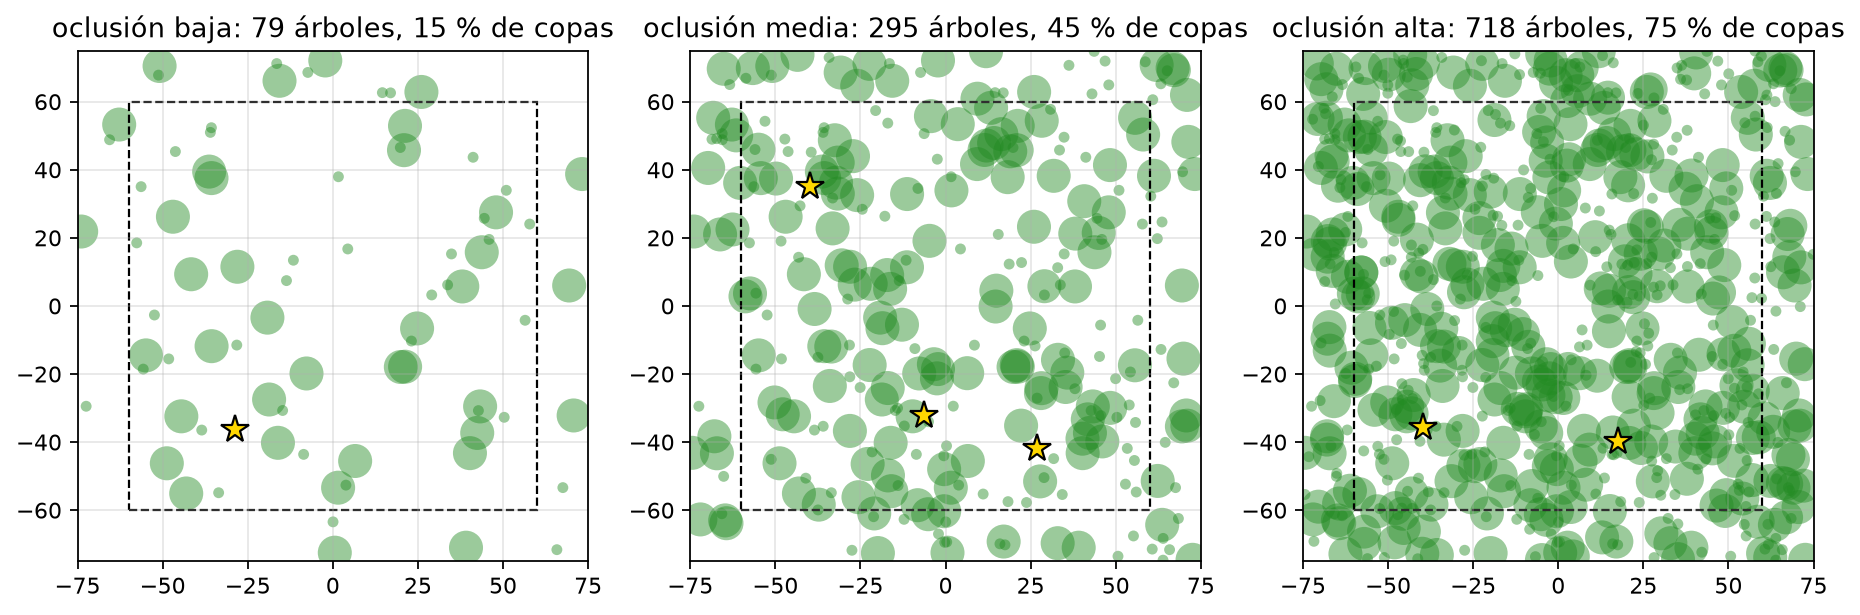
\includegraphics[width=\textwidth]{bosques_oclusion.png}
\caption{Los tres niveles de oclusión con la misma semilla: 79, 295 y 718 árboles. Las estrellas son
las personas.}
\end{figure}

\begin{nota}
Las densidades fijas del diseño original (60, 160 y 280 árboles por hectárea) suponían copas de 6~m; con
los robles de Gazebo Fuel (10~m) daban otra cobertura. Por eso aquí el nivel se define por la cobertura
medida, que es lo que de verdad importa para la cámara, y la densidad resultante se guarda en el JSON.
\end{nota}

\section{Las personas}

De una a tres personas (o las que se pidan con \cod{personas:=}), en posiciones al azar a más de 10~m
del borde, en tres poses: de pie, sentada o acostada. Sus posiciones exactas se guardan en
\cod{personas_<mundo>.json}: la ``verdad'' contra la que se miden los resultados, que la misión nunca
usa para decidir.

\begin{figure}[H]
\centering
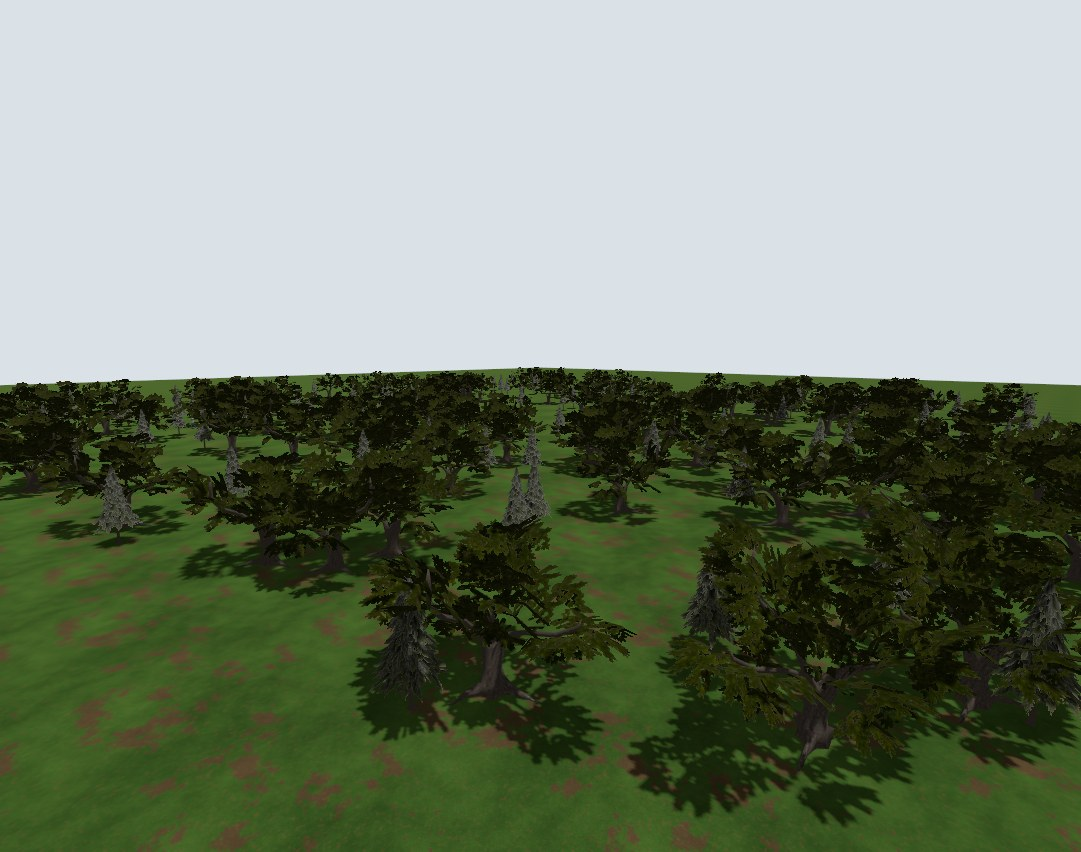
\includegraphics[width=0.8\textwidth]{gz_bosque_bajo.jpg}
\caption{El bosque de oclusión media visto a baja altura.}
\end{figure}

\section{Georreferencia}

Cada mundo declara su ubicación en la Tierra:
\begin{lstlisting}[style=xml]
<spherical_coordinates>
  <surface_model>EARTH_WGS84</surface_model>
  <world_frame_orientation>ENU</world_frame_orientation>
  <latitude_deg>19.4826</latitude_deg>
  <longitude_deg>-99.2447</longitude_deg>
  <elevation>2250</elevation>
</spherical_coordinates>
\end{lstlisting}
Con eso el GPS simulado de PX4 da coordenadas reales, el \emph{home} de ArduPilot se pone en el mismo
punto, y los avisos de personas (que usan la misma conversión, \cod{mision/geo.py}) coinciden con lo
que muestra el mapa de MAVProxy.
